\documentclass[a4paper,12pt]{article}
\usepackage{graphicx}
\usepackage{verbatim}
\usepackage{amsmath}
\begin{document}
	\title{\textbf{Homework1 Rostagno File2}}
	\author{295706}
	\date{\today}
	\maketitle
	
\centering \textbf{Esercizio 1}\\
\begin{itemize}
	\item \textbf{Punto 1}: Dopo aver impostato correttamente i parametri forniti, ho simulato un campione di 1000 elementi come richiesto di una Bernulli. Successivamente ho simulato un campione di una poisson o un campione di una gamma in base se fosse presente un 1 o uno 0 in ogni posizione del campione Bernoulli. Infine ho plottato la cdf tramite il comando R ecdf().
	\begin{figure}[h] % L'ambiente figure permette di gestire il posizionamento
		\centering % Centra l'immagine
		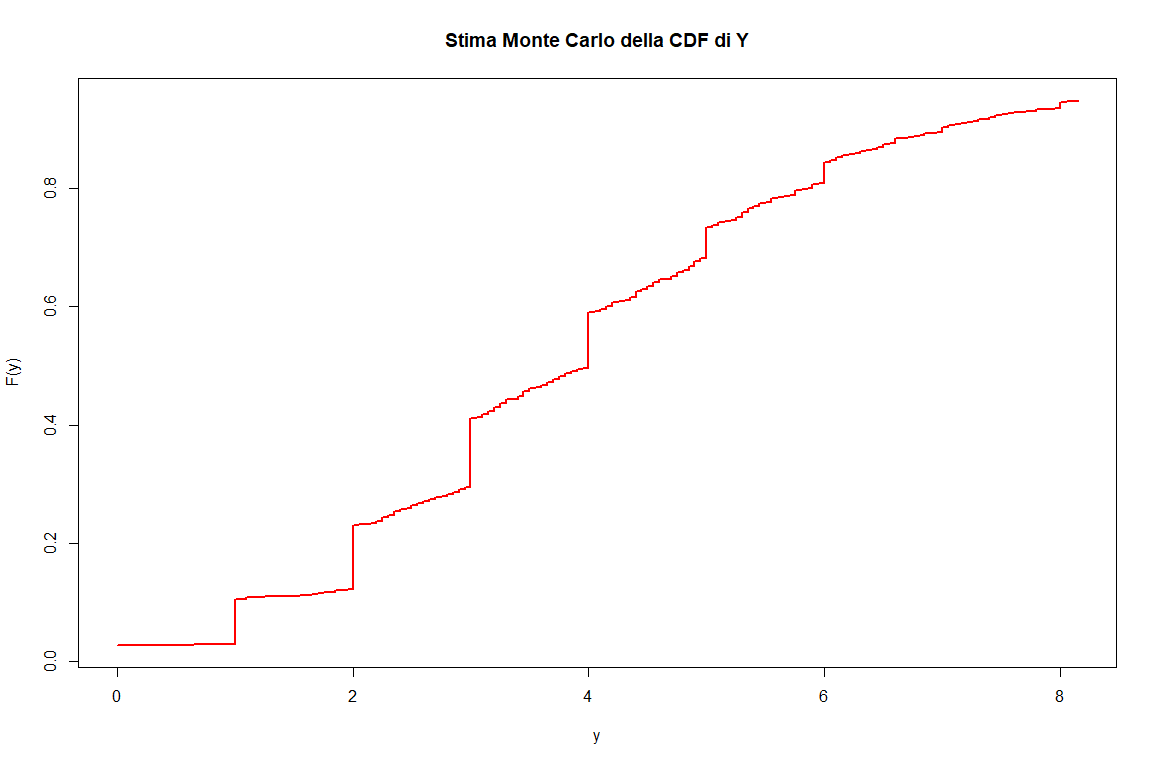
\includegraphics[width=0.8\textwidth]{fRip.png} % Inserisce l'immagine con larghezza metà pagina
		\caption{Stima monte carlo della CDF} % Aggiunge una didascalia all'immagine
		\label{fig:immagine} % Aggiunge un'etichetta per riferimenti interni
	\end{figure}
	\item  \textbf{Punto 2} : Una volta ottenuto il vettore campione Y, ho calcolato la probabilità che gli elementi del vettore fossero fossero presenti nell'intervallo richiesto. Di conseguenza ho contato quanti valori di Y fossero presenti nell'intervallo e ho diviso per il numero totale di elementi del vettore. Stesso procedimento eseguito per il secondo intervallo condizionato,con la differenza che qua ho usato solo gli elementi di Y generati dagli elementi di Z uguali a 0.\\
	Ho ottenuto che la prima probabilità vale 0.173 mentre la seconda vale 0.172. Plausibile in quanto il vettore Z è una Bernoulli di probabilità 0.5. 
	Successivamente devo stimare la varianza, possiamo dire che se un campione cade nell'intervallo è un successo altrimenti no, quindi come una Bernoulli. Di conseguenza la varianza di una Bernoulli è $Var = p \cdot(1-p)$ ed essendo applicata su n campioni diventa: $\hat{Var} =\frac{p \cdot(1-p)}{n}  $, dove p rappresenta le due probabilità precedentemente calcolate. Ottengo che la prima varianza vale 0.000143071, mentre la seconda vale 0.0002756526.
	\item \textbf{Punto 3}: Devo nuovamente calcolare delle probabilità condizionate, ma sta volta uso il teorema di Bayes che nel nostro caso diventa:\\
	\[
	f(Z = 0 \mid Y \in [1.5, 3.5])=\frac{f(Y \in [1.5, 3.5] \mid Z = 0 ) \cdot f(Z = 0)}{f(Y \in [1.5, 3.5])}
	\]
	Quindi calcolo singolarmente le varie probabilità e ottengo nel caso Z=0 una probabilità di 0.6353276, mentre nel caso di Z=1 ottengo 0.3646724. Ovviamente sommano a 1.
	\item \textbf{Punto 4}: Ho semplicemente calcolato i quantili di Y e Z tramite il comando quantile(). \\
	
	Ottenendo per Y i seguenti quantili:\\
	
	\begin{tabular}{|c|c|c|c|}
		\hline
		10\% & 20\% & 50\% & 75\% \\
		\hline
		1.000000 & 2.000000 & 3.986440 & 5.237517 \\
		\hline
	\end{tabular}\\
	
		Ottenendo per Z i seguenti quantili:\newline
	\begin{tabular}{|c|c|c|c|}
		\hline
		10\% & 20\% & 50\% & 75\% \\
		\hline
		0 & 0 & 0 & 1 \\
		\hline
	\end{tabular}
	\item \textbf{Punto 5}: Dato un vettore di punti y, devo calcolare rispetto ai campioni poisson e gamma separatamente la probabilità di ottenerli. Creo un ciclo per i Poisson e ottengo un vettore la probabilità di ottenere ciascun punto del vettore y. Creo un ciclo per i gamma e ottengo la stessa cosa, in questo caso però ho dovuto utilizzare una tolleranza di 0.1 poichè siamo nel caso continuo. Infine plotto le due densità:
	\begin{figure}[h] % L'ambiente figure permette di gestire il posizionamento
		\centering % Centra l'immagine
		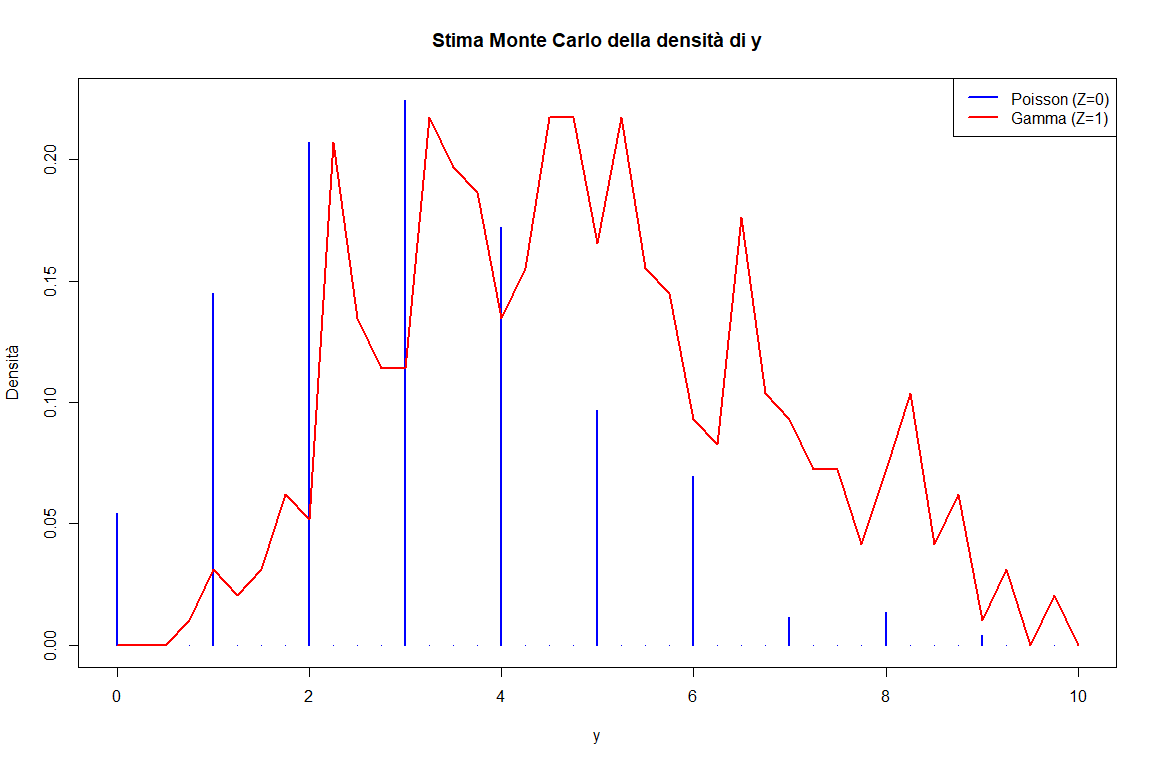
\includegraphics[width=0.8\textwidth]{doppiadens.png} % Inserisce l'immagine con larghezza metà pagina
		\caption{Stima monte carlo della gamma e della Poisson} % Aggiunge una didascalia all'immagine
		\label{fig:immagine} % Aggiunge un'etichetta per riferimenti interni
	\end{figure}	
\end{itemize}
\newpage
\centering \textbf{Esercizio 2}\\
\begin{itemize}
	\item \textbf{Punto 1}: Imposto i vari parametri iniziali e scrivo le funzioni della logistic-normal. Per trovare il valore massimo da usare nel metodo accept-reject ho utilizzato il comando optimize(). Dopodichè ho impostato un ciclo while che mi trovasse n=10 campioni come da richiesta. Simulo le variabili y e u come uniformi nei corrispettivi intervalli $[a,b] $ e $[0,M_1]$. Infine imposto la condizione che se il valore di u è minore della funzione calcolata in y allora accetto y come campione. Il campione da me ottenuto è:\\
	\[
	\left[
	\begin{array}{l}
		0.5248998, 0.9051011, 0.6753934, 0.9386260, \\
		0.4489482, 0.6732017, 0.9271019, 0.7919059, \\
		0.8590266, 0.8970273
	\end{array}
	\right]
	\]
	Successivamente ho svolto un plot grafico generale su 10000 simulazioni imitando quello che è stato mostrato a lezione.
	\begin{figure}[h] % L'ambiente figure permette di gestire il posizionamento
		\centering % Centra l'immagine
		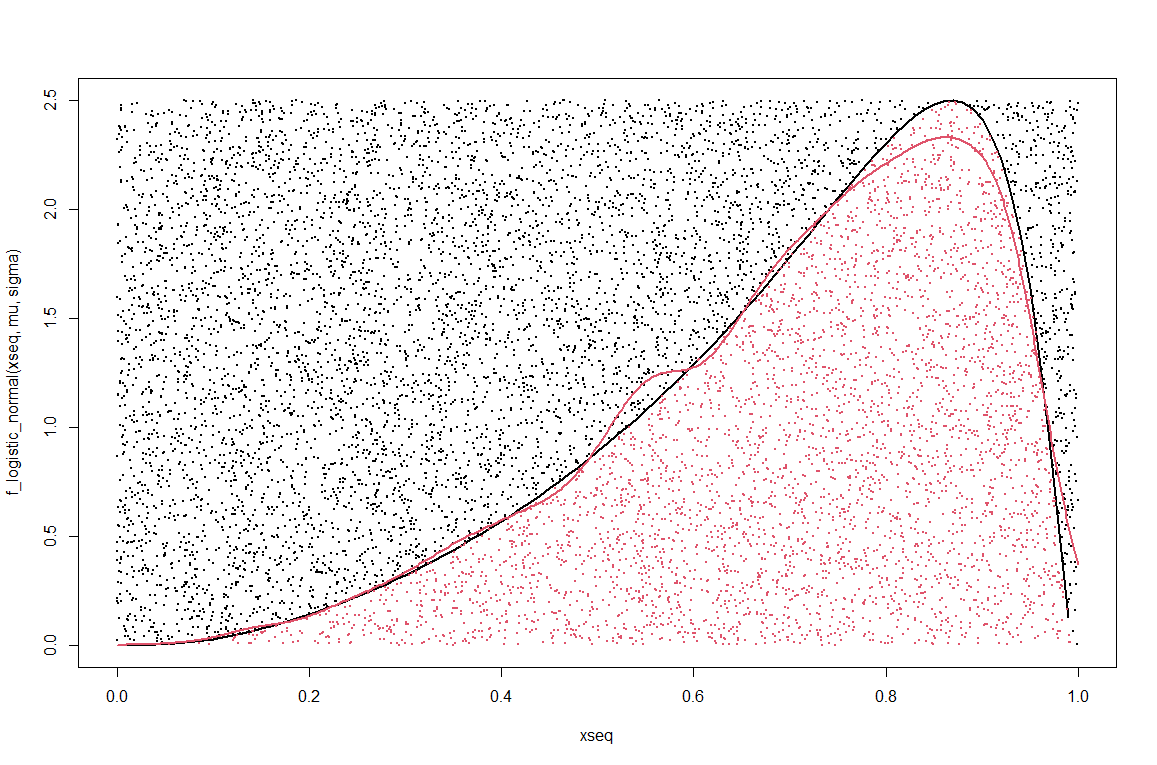
\includegraphics[width=0.8\textwidth]{lognorm.png} % Inserisce l'immagine con larghezza metà pagina
		\caption{campioni accettati e non} % Aggiunge una didascalia all'immagine
		\label{fig:immagine} % Aggiunge un'etichetta per riferimenti interni
	\end{figure}
	\newpage
	\item \textbf{Punto 2}: Imposto la prior di mu e la verosomiglianza in modo da poter ottenere la a posteriori di mu secondo questa proporzione:
	\[
	f(\mu \mid x) \propto f(x \mid \mu) f(\mu)
	\]
	Per calcolare la verosomiglianza ho utilizzato la funzione sapply() che mi permetteva di calcolare per ogni campione la logistic-normal in modo da farne poi il prodotto. Ho utilizzato la log-verosomiglianza per problemi sui numeri(a volte mi dava tutti zeri).\\
	Infine ho plottato la a posteriori di $\mu$:
	\begin{figure}[h] % L'ambiente figure permette di gestire il posizionamento
		\centering % Centra l'immagine
		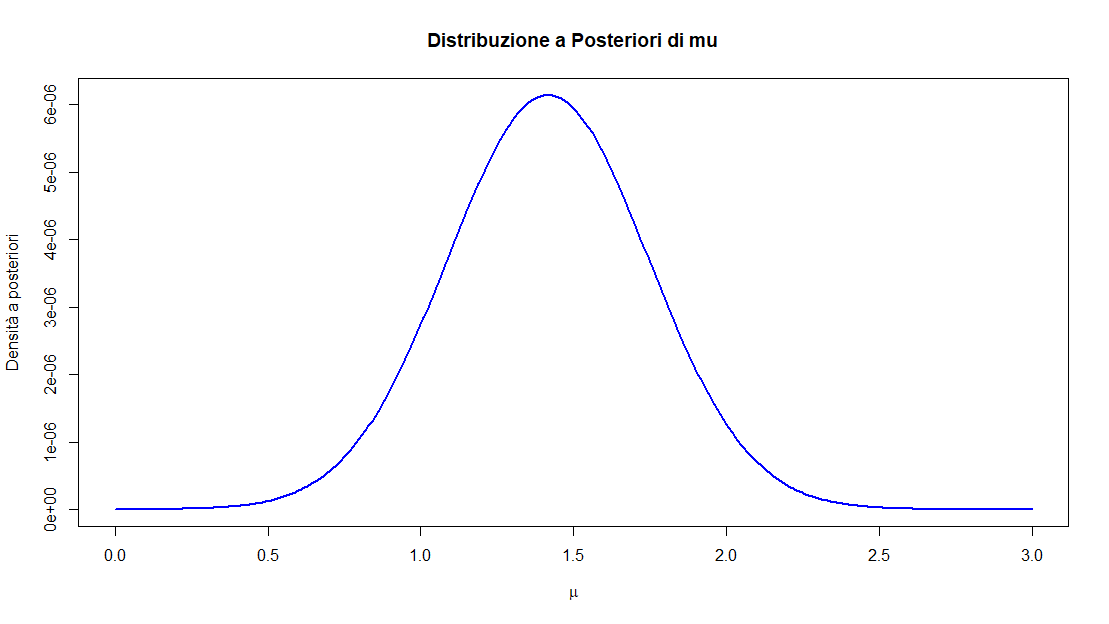
\includegraphics[width=0.8\textwidth]{post.png} % Inserisce l'immagine con larghezza metà pagina
		\caption{Posteriori di $\mu$ con 10 campioni} % Aggiunge una didascalia all'immagine
		\label{fig:immagine} % Aggiunge un'etichetta per riferimenti interni
	\end{figure}
	\newpage
	Successivamente ho ricalcolato il massimo della funzione con optimize() e generato nuovamente delle variabili uniformi negli intervalli $[0,3]$ e $[0,M_2]$. Dopodiche ho verificato la condizione del metodo accept-reject e su 10000 simulazioni ne sono state accettate 2727. Infine ho nuovamente plottato la a posteriori con le varie simulazioni:
	\begin{figure}[h] % L'ambiente figure permette di gestire il posizionamento
		\centering % Centra l'immagine
		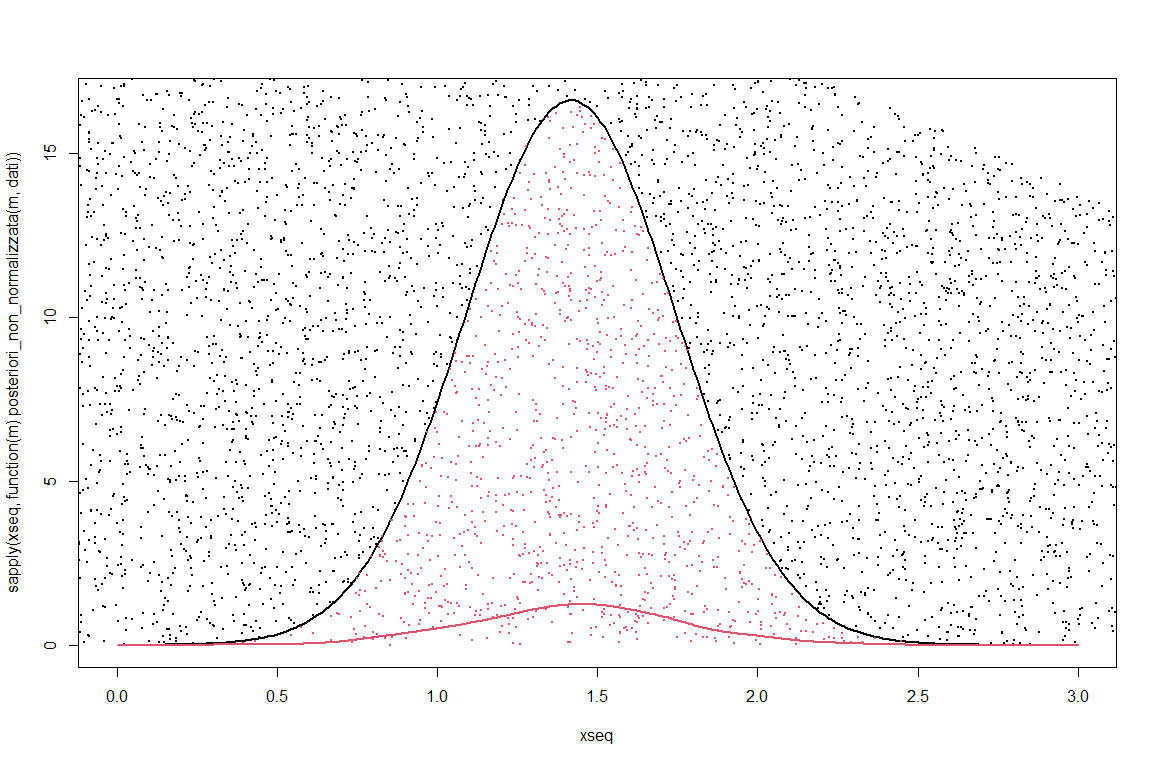
\includegraphics[width=0.8\textwidth]{post2.png} % Inserisce l'immagine con larghezza metà pagina
		\caption{Posteriori di $\mu$ con 10000 simulazioni} % Aggiunge una didascalia all'immagine
		\label{fig:immagine} % Aggiunge un'etichetta per riferimenti interni
	\end{figure}
	\newpage
	\item \textbf{Punto 3}:Ho ripetuto gli stessi passaggi del punto 1 solamente che sta volta ho ottenuto n=100 campioni.\\
	\begin{center}
		\begin{tabular}{|c|c|c|c|c|c|}
			\hline
			0.7519205 & 0.5881544 & 0.9404489 & 0.8170014 & 0.8044540 & 0.6936061 \\
			\hline
			0.3220384 & 0.6206862 & 0.8668681 & 0.8343941 & 0.7431865 & 0.8395818 \\
			\hline
			0.4457116 & 0.7939180 & 0.7037669 & 0.2683472 & 0.9384173 & 0.8597782 \\
			\hline
			0.8504673 & 0.6986789 & 0.8230364 & 0.2825807 & 0.6507637 & 0.7686445 \\
			\hline
			0.6195584 & 0.8676528 & 0.3963593 & 0.8223757 & 0.9525271 & 0.8349073 \\
			\hline
			0.6702257 & 0.3384507 & 0.8555560 & 0.7313662 & 0.8793952 & 0.4595126 \\
			\hline
			0.4673837 & 0.5511715 & 0.9426912 & 0.8801333 & 0.9472494 & 0.7564934 \\
			\hline
			0.6366217 & 0.7724653 & 0.5748576 & 0.7193799 & 0.8518997 & 0.6583162 \\
			\hline
			0.6593640 & 0.5223830 & 0.8117120 & 0.4838693 & 0.5465645 & 0.6496274 \\
			\hline
			0.3464938 & 0.7902977 & 0.8326690 & 0.4742612 & 0.8156803 & 0.4158713 \\
			\hline
			0.6523458 & 0.9802073 & 0.8395061 & 0.4547318 & 0.9198564 & 0.7711883 \\
			\hline
			0.7073175 & 0.6153744 & 0.5216030 & 0.5210493 & 0.7945621 & 0.8267510 \\
			\hline
			0.6235714 & 0.7779817 & 0.5614645 & 0.8361606 & 0.8083573 & 0.9204226 \\
			\hline
			0.9395934 & 0.9243186 & 0.8968904 & 0.4723443 & 0.6836072 & 0.7331385 \\
			\hline
			0.5289565 & 0.3719082 & 0.7550035 & 0.8424244 & 0.4989451 & 0.7289479 \\
			\hline
			0.9149938 & 0.8464283 & 0.3580351 & 0.3558162 & 0.7862829 & 0.1810185 \\
			\hline
			0.8200730 & 0.9766341 & 0.5195689 & & & \\
			\hline
		\end{tabular}
	\end{center}
	Successivamente ho ripetuto i passaggi del punto 2 ma ricalcolando il massimo e adattando la a posteriori ai nuovi campioni.
	Ho ottenuto 1264 campioni accettati e la nuova a posteriori diventa:
	\begin{figure}[h] % L'ambiente figure permette di gestire il posizionamento
		\centering % Centra l'immagine
		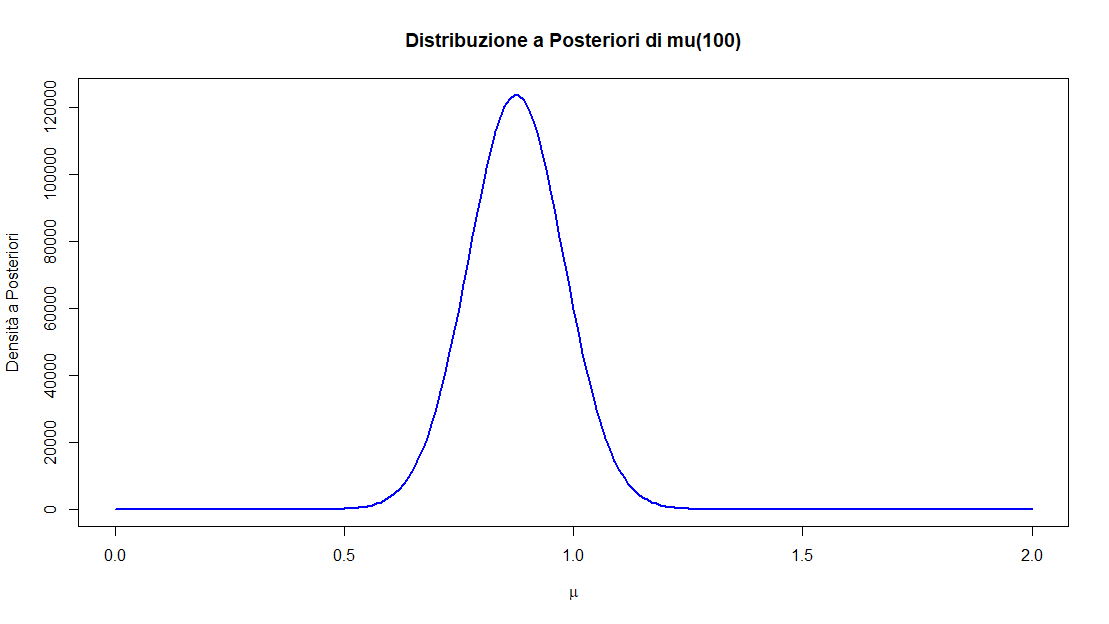
\includegraphics[width=0.8\textwidth]{newpost.png} % Inserisce l'immagine con larghezza metà pagina
		\caption{Posteriori di $\mu$ con 100 campioni} % Aggiunge una didascalia all'immagine
		\label{fig:immagine} % Aggiunge un'etichetta per riferimenti interni
	\end{figure}
	\newline
	Infine ho plottato la prior di $\mu$ in modo da poterla paragonare con le due a posteriori:
	\begin{figure}[h] % L'ambiente figure permette di gestire il posizionamento
		\centering % Centra l'immagine
		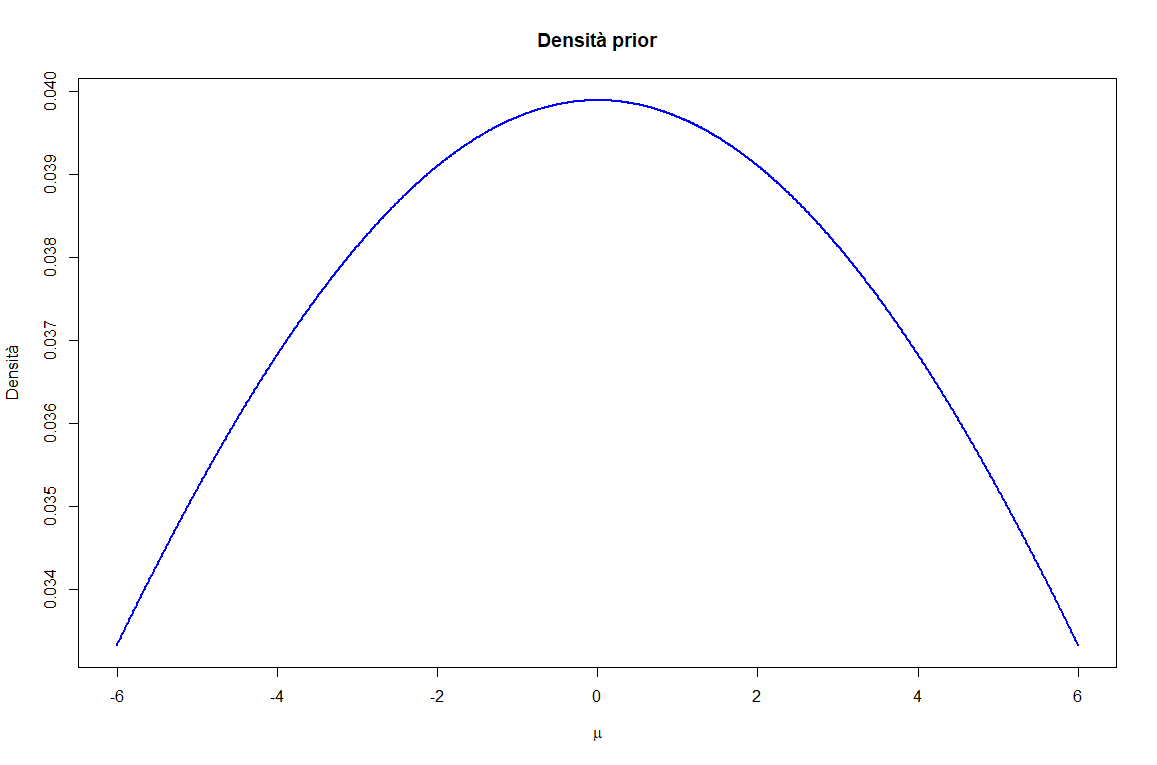
\includegraphics[width=0.8\textwidth]{prior.png} % Inserisce l'immagine con larghezza metà pagina
		\caption{Prior di $\mu$} % Aggiunge una didascalia all'immagine
		\label{fig:immagine} % Aggiunge un'etichetta per riferimenti interni
	\end{figure}
	\newpage
	\item \textbf{Punto 4}: Imposto i parametri dati e ottengo un campione di una Beta(1.2,1.2) con il comando rbeta().
	Successivamente applico il metodo dell’importance sampling che consiste nello stimare $E(X)$ tramite la formula:
	\[
	\frac{\sum_{i=1}^{n} \frac{h(x_i) f(x_i)}{g(x_i)}}{n} \approx E_g \left( \frac{h(X) f(X)}{g(X)} \right) = E_f(h(X))
	\]
	Dove $h(x_i)=x_i$ \\
	$f(x_i)$ è la nostra logistic-normal\\
    $g(x_i)$ è la densità della nostra beta\\
    $n$ è il numero di campioni \\
    $x_i$ sono i valori campionati dalla beta\\
    
    Quindi sostituisco con i miei valori e ottego che l'attesa di X è 0.7486497.
\end{itemize}

\end{document}
